% =====================================================================
%  5. HACIA LA LÓGICA EPISTÉMICA: LOS NIÑOS EMBARRADOS
% =====================================================================
\chapter{Hacia la lógica epistémica: el problema de los niños embarrados}
\label{sec:muddy}

La idea de este capítulo es aterrizar la formalización abstracta de la lógica modal en un ejemplo. Usaremos un acertijo clásico de razonamiento sobre el conocimiento, el llamado problema de los \emph{niños embarrados} (\emph{muddy children}). Presentaremos el problema y algunas de las preguntas que
plantea y haremos una modelización coherente con el desarrollo de los capítulos anteriores con la que demostrar la solución. AAA Lean?

AAA USO DE IA EN 3 SITIOS CONCRETOS IMPORTANTES: GUÍA PARA MODELIZAR (\ref{sec:epistemica}) SIN MODELO MULTIAGENTE COMO EN LA LITERATURA, OBSERVACIÓN \ref{obs:anuncio}, MODELIZACIÓN DE LA PROPOSICIÓN \ref{prop:rondas} DESDE \cite{fhmv}

\section{El acertijo}\label{sec:acertijo}

Un enunciado posible del problema es el siguiente:

\vspace{3mm}

\emph{Hay un grupo de $n$ niños jugando en el jardín. Cuando terminan de jugar, hay $k \ge 1$ de ellos que tienen su frente manchada de barro. Un adulto se acerca al jardín y reúne a los $n$ niños en círculo, de forma que todos los niños pueden ver las frentes de los demás pero no la suya propia.}\footnote{Se entiende que un niño no puede saber si su frente está manchada inicialmente. No puede tocársela o notarse el barro en la frente.} \emph{Posteriormente anuncia:}

\begin{quote}
  \emph{``Al menos uno de vosotros tiene la frente manchada.''}
\end{quote}

\emph{A continuación pregunta:}

\begin{quote}
  \emph{``¿Sabe alguno de vosotros, con certeza, si su propia frente está manchada?''}
\end{quote}

\emph{Los niños que lo sepan deben decir ``sí'' en voz alta, todos a la vez; los demás guardan silencio. Si alguien dice que sí, el juego termina. Si nadie dice nada, el adulto repite la misma pregunta de forma sucesiva (como si fueran turnos o rondas) hasta que algún niño responda. ¿Pueden los niños, sin intercambiar más información que sus propias respuestas, llegar a la conclusión de si su frente está o no manchada?}

\vspace{3mm}

Si suponemos que

\begin{itemize}
    \item todos los niños son lógicos perfectos y capaces de realizar cualquier deducción válida a partir de la información que se presenta;
    \item cada niño es sincero, entendiendo sinceridad como silencio salvo certeza deductiva: un niño dice ``sí'' exactamente cuando ha deducido el estado de su propia frente, y calla en caso contrario;
    \item existe simultaneidad en la recepción de información. Todos oyen a la vez y todos responden a la vez en cada ``turno de pregunta'';
    \item y, todo lo anterior, junto con el enunciado del problema, es \emph{conocimiento común} entre los niños: todos lo saben, todos saben que todos lo saben, todos saben que todos saben que todos lo saben, y así sucesivamente,
\end{itemize}

entonces, la respuesta al acertijo es que sí pueden llegar a una conclusión sobre su frente y, en concreto:

\begin{quote}
  \textbf{En las primeras $k-1$ rondas ningún niño dirá nada. En la ronda $k$, los $k$ niños manchados dirán que sí, y los limpios seguirán en silencio.}
\end{quote}

El último de los supuestos merece atención, y volveremos sobre él en la sección \ref{sec:comun}: no basta con que todos los niños sepan las reglas, hace falta la torre de conocimiento de ``todos saben que todos saben\dots''. Por el momento, los primeros casos pueden verse a mano.

\begin{itemize}
    \item Si $k=1$, el único niño manchado ve todo el resto de frentes limpias. Como el adulto ha dicho que hay al menos una manchada y no es ninguna de las que ve, tiene que ser la suya, y contesta que sí en la primera ronda.
    \item Si $k=2$, cada uno de los dos niños manchados ve una sola frente sucia y ninguno sabe nada de la suya, así que en la primera ronda nadie dice nada. Pero entonces uno razona: ``si yo estuviera limpio, el otro manchado no habría visto ninguna frente manchada y habría contestado que sí. Como ha callado, yo estoy manchado''. El otro niño manchado razona de la misma forma y ambos contestan que sí en la segunda ronda.
    \item Con $k=3$ el argumento se repite un nivel más arriba: cada niño manchado ve dos frentes sucias, espera que esos dos contesten que sí en la segunda ronda y, al ver que callan, deduce que él también está manchado.
\end{itemize}

Esta idea será la que formalizaremos en el resto del capítulo.

Además del razonamiento hacia la solución, el problema deja una paradoja aparente para cualquier caso con $k \ge 2$. En cualquier supuesto así, cada niño ve al menos una frente con barro, de modo que antes de que el adulto informase sobre la existencia de alguna frente manchada, todos los niños ya lo sabían. El anuncio del adulto no parece informar a nadie de nada. Sin embargo, el anuncio es necesario. Sin él, en la situación con $k=2$ el razonamiento del primer niño no se iniciaría, porque no hay ninguna razón para que el segundo hubiera dicho nada en la primera ronda aunque él estuviera limpio. La respuesta a esta paradoja está en el último de los supuestos que hemos escrito, y profundizaremos en ella en la sección \ref{sec:comun}, cuando tengamos el modelo construido. Veremos que existen diferencias entre conocimiento mutuo y conocimiento común.

El acertijo circula en muchas versiones (damas con la cara tiznada, sombreros de colores, sabios y sellos, esposas infieles). Una de las más antiguas del siglo XX es la de Littlewood \cite[pp.~3--4]{littlewood}, planteada con tres damas que viajan en un vagón de tren y que además la generaliza a $n$ damas y resuelve el caso general por inducción. El tratamiento estándar, con la terminología de los niños embarrados, es el del capítulo 1 de \cite{fhmv}. La lectura dinámica que seguimos aquí, en la que cada anuncio transforma el modelo, es la de \cite{ditmarsch}.

\section{El conocimiento como modalidad}\label{sec:epistemica}

La tabla \ref{tab:lecturas} del capítulo \ref{sec:logicamodal} anunciaba la lectura epistémica de $\nec$: ``$\varphi$ se sabe''. Pero saber es algo que alguien hace. A ese ``alguien'', en el contexto de la lógica epistémica, se le conoce como \emph{agente}.

Fijemos entonces un agente. Sus mundos posibles son las descripciones completas de cómo podría ser la realidad, y la relación de accesibilidad se lee ahora como una relación de \emph{indistinguibilidad}: $w \sim v$ significa que, si $v$ fuera el estado real del mundo, el agente tendría exactamente las mismas observaciones que tiene en $w$, de modo que no puede diferenciarlo y, por ende, descartarlo. Con esa lectura, la cláusula de la definición de satisfacción \ref{def:satisfaccion},
\[
  M, w \vDash \nec\varphi \iff \text{para todo } v \text{ con } w \sim v,\ M, v \vDash \varphi,
\]
dice que $\varphi$ es verdadera en todos los estados que el agente considera posibles, es decir, que $\varphi$ se sigue de lo que observa. Esto es lo que llamamos \emph{saber} $\varphi$. La fórmula dual, $\pos\varphi$, dice que hay un estado compatible con sus observaciones en el que $\varphi$ es cierta. Esto es que el agente \emph{considera posible} $\varphi$. En la lectura epistémica es habitual escribir $K\varphi$ y $\widehat{K}\varphi$ (de \emph{knowledge}) en lugar de $\nec\varphi$ y $\pos\varphi$, pero se trata de los mismos operadores.

Cuando hay varios agentes, cada uno tiene su propia relación de indistinguibilidad sobre los mismos mundos. El tratamiento estándar las reúne en un solo modelo multiagente, con una relación $\sim_i$ y un operador $K_i$ por agente, sobre un lenguaje con tantas cajas como agentes \cite[cap.~2]{fhmv}. Nosotros no podemos hacer exactamente eso, porque tanto el lenguaje del capítulo \ref{sec:logicamodal} como su formalización del capítulo \ref{sec:formalizacion} tienen una sola caja. Pero obsérvese qué es realmente un modelo multiagente: \emph{una familia de modelos de Kripke con los mismos mundos y la misma valoración, uno por agente}. Y una fórmula del fragmento monoagente, esto es, una en la que aparece el operador de un único agente, se evalúa enteramente dentro del modelo de ese agente. Por eso, en todo este capítulo, en lugar de definir un lenguaje nuevo escribiremos
\[
  M^{(i)}, S \vDash \nec\varphi
\]
para decir que el niño $i$ sabe $\varphi$, donde $M^{(i)}$ es el modelo de Kripke cuya relación de accesibilidad es la indistinguibilidad de $i$. El lenguaje, los modelos y la satisfacción son los de los capítulos \ref{sec:logicamodal} y \ref{sec:formalizacion}, sin ningún cambio.

El problema que trae esta decisión es que no se pueden escribir fórmulas que mezclen el conocimiento de dos niños, como $K_1K_2\varphi$. Para el teorema \ref{teo:muddy} no hace falta, pues en él solo aparecen $\nec m_i$ y $\nec\lnot m_i$ para un niño cada vez. Sí hará falta, en cambio, para el anuncio de la sección \ref{sec:anuncios} y para la discusión del conocimiento común de la sección \ref{sec:comun}. En ambos casos lo señalaremos explícitamente y explicaremos cómo se suple.

\section{El modelo del acertijo}\label{sec:modelo-ninos}

Para construir el modelo hay que decidir tres cosas: qué es un mundo posible, cuándo dos mundos son indistinguibles para cada niño y qué variables son verdaderas en cada mundo. Un mundo debe describir por completo lo que puede variar. Pero lo único que varía es quién está manchado, por tanto, un mundo es un subconjunto de $N = \{1,\dots,n\}$, y hay $2^n$. El niño $i$ ve todas las frentes menos la suya, de modo que no puede distinguir dos mundos que coincidan en todo salvo en él mismo. Y la variable $m_i$, ``el niño $i$ está manchado'', es verdadera en el mundo $S$ exactamente cuando $i \in S$.

\begin{definicion}[El cubo]\label{def:cubo}
Sea $N = \{1,\dots,n\}$ y sea $\mathsf{VP} = \{m_1,\dots,m_n\}$. Para cada niño $i$, sea $M^{(i)} = (W, \sim_i, V)$ el modelo de Kripke dado por
\[
  W = \mathcal{P}(N), \qquad
  S \sim_i T \iff S \setminus \{i\} = T \setminus \{i\}, \qquad
  V(S) = \{ m_j : j \in S \}.
\]
Los mundos y la valoración son los mismos para todos los niños. Lo que cambia de un modelo a otro es la relación de accesibilidad. El \emph{mundo real} $S^{*}$ es el conjunto de los niños que están efectivamente manchados, y $k = |S^{*}|$.
\end{definicion}

El nombre de \emph{cubo} viene de la forma del modelo. Si identificamos cada subconjunto con su vector característico, los mundos son los vértices del cubo $\{0,1\}^n$ y las aristas de la dirección $i$ son los pares relacionados por $\sim_i$. La figura \ref{fig:cubo} lo dibuja para $n=3$, superponiendo los tres modelos en un solo diagrama.

\begin{figure}[htb]
\centering
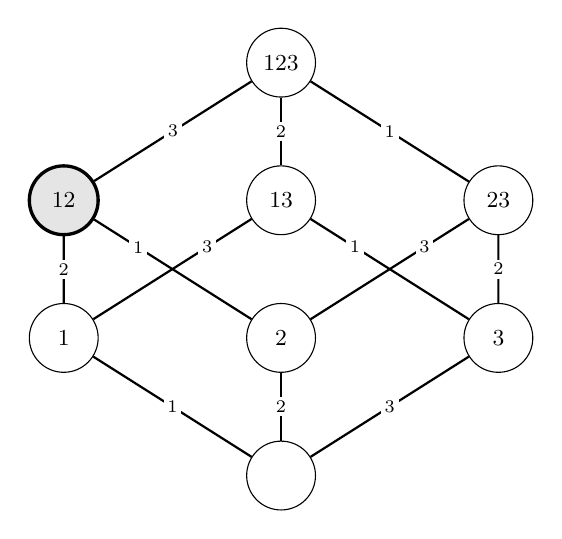
\begin{tikzpicture}[scale=0.92, transform shape,
    mundo/.style={circle, draw, minimum size=0.95cm, inner sep=1pt, font=\small},
    actual/.style={mundo, very thick, fill=black!10},
    arista/.style={thick},
    etiq/.style={font=\scriptsize, inner sep=1.5pt, fill=white}]
  \node[mundo]  (v0)   at (0,0)     {$\varnothing$};
  \node[mundo]  (v1)   at (-3,1.9)  {$1$};
  \node[mundo]  (v2)   at (0,1.9)   {$2$};
  \node[mundo]  (v3)   at (3,1.9)   {$3$};
  \node[actual] (v12)  at (-3,3.8)  {$12$};
  \node[mundo]  (v13)  at (0,3.8)   {$13$};
  \node[mundo]  (v23)  at (3,3.8)   {$23$};
  \node[mundo]  (v123) at (0,5.7)   {$123$};
  \draw[arista] (v0) -- node[etiq]{$1$} (v1);
  \draw[arista] (v0) -- node[etiq]{$2$} (v2);
  \draw[arista] (v0) -- node[etiq]{$3$} (v3);
  \draw[arista] (v1) -- node[etiq]{$2$} (v12);
  \draw[arista] (v2) -- node[etiq, pos=0.72]{$1$} (v12);
  \draw[arista] (v1) -- node[etiq, pos=0.72]{$3$} (v13);
  \draw[arista] (v3) -- node[etiq, pos=0.72]{$1$} (v13);
  \draw[arista] (v2) -- node[etiq, pos=0.72]{$3$} (v23);
  \draw[arista] (v3) -- node[etiq]{$2$} (v23);
  \draw[arista] (v12) -- node[etiq]{$3$} (v123);
  \draw[arista] (v13) -- node[etiq]{$2$} (v123);
  \draw[arista] (v23) -- node[etiq]{$1$} (v123);
\end{tikzpicture}
\caption{Los modelos $M^{(1)}$, $M^{(2)}$ y $M^{(3)}$ para $n=3$, dibujados a la vez. Cada mundo se nombra por el conjunto de niños manchados ($12$ abrevia $\{1,2\}$) y cada arista lleva la etiqueta del niño que no distingue sus extremos, de modo que el modelo del niño $i$ es el que resulta de quedarse solo con las aristas etiquetadas con $i$. Se omiten los bucles $S \sim_i S$. Los mundos están dispuestos por niveles según su número de manchados; en gris, el mundo real del ejemplo que seguiremos, $S^{*} = \{1,2\}$.}
\label{fig:cubo}
\end{figure}

El lema siguiente dice que las clases de indistinguibilidad son muy pequeñas. Cada niño duda entre dos mundos y solo dos. Escribimos $S \simdif \{i\}$ (la diferencia simétrica de $S$ con el conjunto $\{i\}$) para el mundo que resulta de cambiar en $S$ el estado del niño $i$, esto es, $S \setminus \{i\}$ cuando $i \in S$ y $S \cup \{i\}$ cuando $i \notin S$. Obsérvese que $S \simdif \{i\}$ es siempre distinto de $S$.

\begin{lema}[Vecinos]\label{lema:vecinos}
$S \sim_i T$ si y solo si $T = S$ o $T = S \simdif \{i\}$.
\end{lema}

\begin{proof}
Si $T = S$ o $T = S \simdif \{i\}$, entonces $S$ y $T$ tienen los mismos elementos distintos de $i$, luego $S \sim_i T$. Recíprocamente, sea $S \sim_i T$. Si $i$ pertenece a los dos conjuntos o a ninguno, entonces $S$ y $T$ coinciden también en $i$, y $T = S$. Si pertenece exactamente a uno, digamos $i \in S$ e $i \notin T$, entonces $T = T \setminus \{i\} = S \setminus \{i\} = S \simdif \{i\}$, y análogamente en el otro caso.
\end{proof}

\begin{observacion}[Por qué esto es una lógica del conocimiento]\label{obs:s5}
La relación $\sim_i$ es de equivalencia, pues es el núcleo de la aplicación $S \mapsto S \setminus \{i\}$; por el lema \ref{lema:vecinos}, además, sus clases son exactamente los pares $\{S, S \simdif\{i\}\}$. La sección \ref{sec:kripke-mat} señalaba que ciertas fórmulas son válidas exactamente en los marcos con cierta propiedad. Por ejemplo, $\nec p \limp p$ lo es en los reflexivos. Las tres propiedades que hacen de $\sim_i$ una equivalencia se corresponden, en ese mismo sentido, con tres esquemas:
\[
  \begin{array}{lll}
    \text{reflexiva}  & \text{(T)}\ \ \nec\varphi \limp \varphi
                      & \text{lo sabido es cierto,} \\[2pt]
    \text{transitiva} & \text{(4)}\ \ \nec\varphi \limp \nec\nec\varphi
                      & \text{quien sabe algo sabe que lo sabe,} \\[2pt]
    \text{euclídea}   & \text{(5)}\ \ \lnot\nec\varphi \limp \nec\lnot\nec\varphi
                      & \text{quien no sabe algo sabe que no lo sabe,}
  \end{array}
\]
donde \emph{euclídea} significa que de $w \sim v$ y $w \sim u$ se sigue $v \sim u$. Los dos últimos esquemas se conocen como \emph{introspección positiva} y \emph{negativa}, respectivamente. Las tres propiedades son en realidad redundantes: una relación reflexiva y euclídea es simétrica (de $w \sim v$ y $w \sim w$ se sigue $v \sim w$) y también transitiva (si $w \sim v$ y $v \sim u$, la simetría da $v \sim w$ y la propiedad euclídea aplicada en $v$ da $w \sim u$), luego es de equivalencia; por eso $\mathbf{S5}$ suele axiomatizarse solo con (T) y (5). El sistema $\K$ ampliado con estos esquemas es $\mathbf{S5}$, la lógica epistémica estándar \cite[cap.~3]{fhmv}. Las correspondencias entre esquemas y propiedades de los marcos que acabamos de invocar no se demuestran en este trabajo; son el objeto del capítulo 3 de \cite{blackburn}, como ya se indicó en la sección \ref{sec:kripke-mat}. Tampoco usaremos $\mathbf{S5}$ como sistema, porque en este capítulo no se demuestra nada en un cálculo axiomático y todo son comprobaciones semánticas dentro de un modelo concreto. (AAA SI MUDDY-LEAN, AÑADIR QUE SE VE T)
\end{observacion}

Cerramos la sección con dos comprobaciones sencillas que sirven para convencerse de que el modelo dice lo que queremos.

\begin{itemize}
    \item Cada niño conoce el estado de los demás: si $i \ne j$, las fórmulas $m_j \limp \nec m_j$ y $\lnot m_j \limp \nec\lnot m_j$ son válidas en $M^{(i)}$. Para la primera, de $j \in S$ y $S \sim_i T$ se sigue $j \in S \setminus \{i\} = T \setminus \{i\} \subseteq T$, donde el primer paso usa que $j \ne i$, Para la segunda, de $j \notin S$ y $S \sim_i T$ se sigue $j \notin T$, pues $j \in T$ daría $j \in T\setminus\{i\} = S \setminus\{i\} \subseteq S$.
    \item Ningún niño sabe nada sobre su propia frente: para todo mundo $S$ y todo $i$ se tiene $M^{(i)}, S \nvDash \nec m_i$ y $M^{(i)}, S \nvDash \nec\lnot m_i$, porque $S$ y $S \simdif\{i\}$ son dos mundos indistinguibles para $i$, uno con $m_i$ verdadera y otro con $m_i$ falsa. Dicho con el operador dual, $M^{(i)}, S \vDash \pos m_i \land \pos\lnot m_i$: el niño considera posibles las dos cosas.
\end{itemize}

\section{Cómo los anuncios públicos cambian el modelo}\label{sec:anuncios}

El modelo describe la situación inicial, pero el acertijo es dinámico. Los anuncios del adulto y las respuestas de los niños son sucesos que cambian lo que cada niño sabe.

\begin{definicion}[Restricción]\label{def:restriccion}
Sea $M = (W, R, V)$ un modelo de Kripke y sea $P \subseteq W$ no vacío. El modelo \emph{restringido} $M|_P$ tiene como mundos los de $P$, como relación la restricción $R \cap (P \times P)$ y como valoración la restricción de $V$ a $P$.
\end{definicion}

La condición $P \ne \varnothing$ es la que exige la definición \ref{def:kripke}, y en el acertijo se cumplirá siempre.

Si algo se anuncia en voz alta y es cierto, todos descartan a la vez los estados incompatibles con lo anunciado, y nadie gana ni pierde capacidad de observación, de modo que quien no distinguía dos mundos supervivientes los sigue sin distinguir. Esto no es un teorema, sino la decisión de modelización que define qué entendemos por anuncio público: cuando $P$ es el conjunto de mundos donde una fórmula $\varphi$ es verdadera, $M|_P$ es el modelo actualizado tras anunciar $\varphi$, y es el operador básico de la \emph{lógica de anuncios públicos} de Plaza \cite{plaza} (véase \cite{ditmarsch} para un tratamiento moderno). La restricción se aplica a la vez a los $n$ modelos, porque el anuncio lo oyen todos. Nótese que la definición \ref{def:restriccion} admite cualquier $P$ no vacío, sin exigir que sea el conjunto de verdad de una fórmula; esto será importante enseguida.

Veamos qué anuncios hay en el acertijo. El primero es el del adulto, ``al menos uno de vosotros está manchado'', que es verdadero exactamente en los mundos $S$ con $|S| \ge 1$. Es decir, que elimina un solo mundo, el $\varnothing$. Los siguientes anuncios son las respuestas. Como todos responden a la vez y en voz alta, que nadie diga nada equivale a un único anuncio público, ``ningún niño sabe si está manchado''; y ese anuncio elimina, por definición, los mundos en los que algún niño sí lo sabría. El trabajo consiste en identificar los modelos que van apareciendo.

\begin{observacion}\label{obs:anuncio}
Ese segundo anuncio no es una fórmula de nuestro lenguaje. Escrito con todas las letras sería
\[
  \bigwedge_{i=1}^{n} \bigl(\lnot\nec m_i \land \lnot\nec\lnot m_i\bigr),
\]
pero cada una de sus partes ha de evaluarse en el modelo del niño correspondiente, de modo que la conjunción mezcla los $n$ modelos y no puede formarse en un lenguaje con una sola caja (sección \ref{sec:epistemica}). Esto no impide usarla: la definición \ref{def:restriccion} solo necesita un subconjunto de $W$, y
\[
  P \;=\; \bigl\{\, S \in W \;:\; \text{para todo } i,\
  M^{(i)}, S \nvDash \nec m_i \ \text{y}\ M^{(i)}, S \nvDash \nec\lnot m_i \,\bigr\}
\]
es un subconjunto de $W$ perfectamente determinado, definido en el metalenguaje a partir de condiciones que sí son monoagentes. Lo que perdemos es la posibilidad de \emph{escribir} el anuncio como una fórmula del lenguaje objeto; en un modelo multiagente sería una fórmula más, y así es como lo presenta el tratamiento estándar \cite[cap.~1]{fhmv}.
\end{observacion}

\begin{definicion}[Escenarios]\label{def:escenarios}
Para $0 \le r \le n$, sea $W_r = \{ S \subseteq N : |S| \ge r \}$ y sea $M_r^{(i)} = M^{(i)}|_{W_r}$. En particular, $W_0 = \mathcal{P}(N)$ y $M_0^{(i)} = M^{(i)}$.
\end{definicion}

La cota $r \le n$ garantiza que $W_r \ne \varnothing$, pues $N \in W_r$ siempre, como exige la definición \ref{def:restriccion}. Obsérvese además que el mundo real sobrevive a todas las restricciones que vamos a usar: si $k = |S^{*}|$, entonces $S^{*} \in W_r$ para todo $r \le k$. Esto es imprescindible, porque un anuncio público solo tiene sentido cuando lo anunciado es verdadero en el mundo real.

Así, $M_0^{(i)}$ es el cubo entero (todo mundo tiene al menos $0$ manchados) y $M_1^{(i)}$ es el modelo tras el anuncio del adulto. El teorema de la sección siguiente demostrará que $M_r^{(i)}$ es el modelo vigente en la ronda $r$-ésima, es decir, el que queda tras el anuncio del adulto y $r-1$ rondas de silencio; en él todos los mundos tienen al menos $r$ manchados, de modo que a esas alturas ningún niño considera ya posible que haya menos de $r$ frentes sucias. El anuncio del adulto borra del cubo de la figura \ref{fig:cubo} el vértice $\varnothing$ y sus tres aristas; obsérvese que, hecho eso, en un mundo de un solo manchado ese niño se queda sin alternativa y sabe que está manchado, que es la razón de que los mundos del primer nivel sean los que la primera ronda de silencio eliminará. La figura \ref{fig:escenario23} muestra los dos escenarios siguientes.

\begin{figure}[htb]
\centering
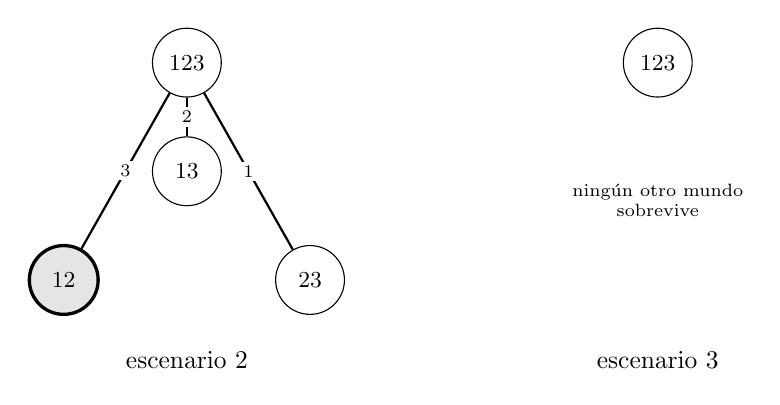
\begin{tikzpicture}[scale=0.92, transform shape,
    mundo/.style={circle, draw, minimum size=0.95cm, inner sep=1pt, font=\small},
    actual/.style={mundo, very thick, fill=black!10},
    arista/.style={thick},
    etiq/.style={font=\scriptsize, inner sep=1.5pt, fill=white}]
  \node[actual] (v12)  at (-1.7,0)   {$12$};
  \node[mundo]  (v13)  at (0,1.5)    {$13$};
  \node[mundo]  (v23)  at (1.7,0)    {$23$};
  \node[mundo]  (v123) at (0,3.0)    {$123$};
  \draw[arista] (v12) -- node[etiq]{$3$} (v123);
  \draw[arista] (v13) -- node[etiq]{$2$} (v123);
  \draw[arista] (v23) -- node[etiq]{$1$} (v123);
  \node at (0,-1.1) {escenario $2$};
  \begin{scope}[xshift=6.5cm]
    \node[mundo] (w123) at (0,3.0) {$123$};
    \node[font=\scriptsize, align=center] at (0,1.1)
      {ningún otro mundo\\ sobrevive};
    \node at (0,-1.1) {escenario $3$};
  \end{scope}
\end{tikzpicture}
\caption{Los escenarios $2$ y $3$ para $n=3$, es decir, los modelos vigentes en las rondas segunda y tercera. En el escenario $2$, el mundo real $\{1,2\}$ solo está conectado con $\{1,2,3\}$, y por la arista del niño $3$: los niños $1$ y $2$ no tienen ya ninguna alternativa y saben que están manchados, mientras que el niño $3$ sigue dudando entre estar limpio (mundo $\{1,2\}$) y estar manchado (mundo $\{1,2,3\}$). Con $k=2$ el juego termina aquí, en la segunda ronda; el escenario $3$ solo llega a ser el modelo vigente si $k=3$.}
\label{fig:escenario23}
\end{figure}

\section{El teorema}\label{sec:teorema-ninos}

Fijemos primero la terminología. Diremos que el niño $i$ \emph{sabe si está manchado} en el mundo $S$ del escenario $r$ cuando
\[
  M_r^{(i)}, S \vDash \nec m_i \lor \nec\lnot m_i,
\]
esto es, cuando sabe que lo está o sabe que no lo está.

La proposición siguiente es el corazón del capítulo: describe exactamente quién sabe qué en cada escenario. Obsérvese que sus tres apartados agotan los casos posibles, pues un mundo $S$ del escenario $r$ cumple $|S| \ge r$ y el niño $i$ está o no está en $S$.

\begin{proposicion}\label{prop:rondas}
Sean $0 \le r \le n$ y $S$ un mundo del escenario $r$, es decir, $|S| \ge r$. Entonces:
\begin{enumerate}
  \item[(a)] si $i \in S$ y $|S| = r$, entonces $M_r^{(i)}, S \vDash \nec m_i$;
  \item[(b)] si $i \in S$ y $|S| > r$, entonces $M_r^{(i)}, S \nvDash \nec m_i$ y $M_r^{(i)}, S \nvDash \nec\lnot m_i$;
  \item[(c)] si $i \notin S$, entonces $M_r^{(i)}, S \nvDash \nec m_i$ y $M_r^{(i)}, S \nvDash \nec\lnot m_i$.
\end{enumerate}
\end{proposicion}

\begin{proof}
Por el lema \ref{lema:vecinos}, los únicos mundos indistinguibles de $S$ para el niño $i$ son $S$ y $S \simdif \{i\}$; toda la demostración consiste en ver cuál de los dos sobrevive en el escenario $r$.

(a) Sea $T$ un mundo del escenario con $S \sim_i T$ y supongamos, por reducción al absurdo, que $i \notin T$. Como $i \in S$, no puede ser $T = S$, luego $T = S \setminus \{i\}$ y $|T| = |S| - 1 = r-1$. Pero $T$ está en el escenario $r$, así que $|T| \ge r$: contradicción (nótese que $r \ge 1$, porque $S$ contiene a $i$ y $|S| = r$). Por tanto $i \in T$ para todo mundo accesible, es decir, $M_r^{(i)}, S \vDash \nec m_i$.

(b) El mundo $T = S \setminus \{i\}$ cumple $|T| = |S| - 1 \ge r$, porque $|S| > r$, luego sigue en el escenario, e $i \notin T$. Como también $S$ está en el escenario e $i \in S$, el niño $i$ considera posibles dos mundos que discrepan sobre $m_i$: en $T$ falla $m_i$, lo que refuta $\nec m_i$, y en $S$ falla $\lnot m_i$, lo que refuta $\nec\lnot m_i$.

(c) El mundo $T = S \cup \{i\}$ cumple $|T| \ge |S| \ge r$, luego sigue en el escenario, e $i \in T$. De nuevo $S$ y $T$ discrepan sobre $m_i$ y ninguno de los dos ha sido eliminado, así que $i$ no sabe nada sobre su propia frente.
\end{proof}

El apartado (c) permite extraer una observación. Un niño limpio nunca averigua que lo está a partir de los anuncios de que nadie sabe nada, por muchas rondas de silencio que pasen. La razón es que el mundo alternativo que él considera posible tiene \emph{más} manchados que el real, y esos anuncios sucesivos no eliminan dichos mundos.\footnote{Cosa distinta es lo que ocurre \emph{después} de la ronda $k$. El niño limpio $i$ habrá oído entonces que los niños de $S^{*}$ sí saben, y ese anuncio elimina el mundo $S^{*}\cup\{i\}$: en él hay $k+1$ manchados y, por los apartados (b) y (c), nadie habría hablado. Al niño $i$ solo le quedaría el mundo $S^{*}$ y sabría que está limpio. Lo que demuestra el apartado (c) es, precisamente, que ningún anuncio de la forma ``nadie lo sabe'' le sirve de nada.}

\begin{corolario}\label{cor:ronda}
Sean $1 \le r \le n$ y $S$ un mundo del escenario $r$. Entonces algún niño sabe si está manchado en $S$ si y solo si $|S| = r$. En consecuencia, si $r < n$, los mundos del escenario $r$ que sobreviven al anuncio ``ningún niño sabe si está manchado'' son exactamente los del escenario $r+1$.
\end{corolario}

\begin{proof}
Si $|S| = r$, como $r \ge 1$ el conjunto $S$ no es vacío; tomando $i \in S$, el apartado (a) da $M_r^{(i)}, S \vDash \nec m_i$. Recíprocamente, si $|S| \ne r$, entonces $|S| > r$ porque $S$ está en el escenario $r$, y los apartados (b) y (c) cubren todos los niños: ninguno sabe nada. Para la segunda parte, sobreviven los mundos con $|S| \ge r$ en los que nadie sabe nada, que son los que cumplen además $|S| \ne r$, es decir, $|S| \ge r+1$; y como las relaciones y la valoración son en ambos casos las de $M^{(i)}$ restringidas, los modelos coinciden.
\end{proof}

Con esto, el acertijo está resuelto: solo queda encadenar las rondas.

\begin{teorema}[Los niños embarrados]\label{teo:muddy}
Supongamos que el mundo real es $S^{*}$ con $k = |S^{*}|$ y $1 \le k \le n$. Entonces, para cada $r$ con $1 \le r \le k$, el modelo vigente en la ronda $r$ es el escenario $r$ y:
\begin{itemize}
  \item si $r < k$, ningún niño sabe si está manchado, y todos guardan silencio;
  \item si $r = k$, los niños de $S^{*}$ saben que están manchados y contestan que sí, y los demás siguen sin saber nada y callan.
\end{itemize}
\end{teorema}

\begin{proof}
Sea $P(r)$ la afirmación ``el modelo vigente en la ronda $r$ es el escenario $r$''. Demostramos $P(r)$ para $1 \le r \le k$ por inducción sobre $r$, y de camino obtenemos las dos viñetas.

\emph{Caso base.} El modelo vigente antes de que nadie hable es el escenario $0$, el cubo entero. El anuncio del adulto es cierto en $S^{*}$, pues $k \ge 1$, y su conjunto de verdad es $W_1$, de modo que la restricción da el escenario $1$: este es el modelo con el que los niños responden a la primera pregunta. Luego $P(1)$.

\emph{Paso inductivo.} Sean $1 \le r < k$ y supongamos $P(r)$. El mundo real cumple $|S^{*}| = k > r$, así que por los apartados (b) y (c) de la proposición \ref{prop:rondas} ningún niño sabe si está manchado y todos guardan silencio; esta es la primera viñeta. Ese silencio conjunto es el anuncio ``ningún niño sabe si está manchado'', cierto en $S^{*}$, y la segunda parte del corolario \ref{cor:ronda} identifica el modelo restringido con el escenario $r+1$, que es por tanto el modelo vigente en la ronda $r+1$. Luego $P(r+1)$.

\emph{Conclusión.} Por $P(k)$, el modelo vigente en la ronda $k$ es el escenario $k$, y $|S^{*}| = k$. El apartado (a) de la proposición \ref{prop:rondas} da $M_k^{(i)}, S^{*} \vDash \nec m_i$ para todo $i \in S^{*}$, y el apartado (c), que ningún niño limpio sabe nada. Esta es la segunda viñeta.
\end{proof}

\section{El anuncio del adulto y el conocimiento común}\label{sec:comun}

Volvamos a la paradoja que dejamos planteada en la sección \ref{sec:acertijo}. Si hay dos o más niños manchados, todos ven al menos una frente sucia, de modo que todos saben ya lo que el adulto va a decirles antes de que abra la boca. Y sin embargo, sin ese anuncio el acertijo no se resuelve. ¿Qué puede aportar una frase que todo el mundo sabe?

La respuesta corta es que el anuncio no informa sobre el barro. Informa sobre lo que los demás saben.

Para verlo, situémonos \emph{antes} de que el adulto hable por primera vez. Tomemos $n=3$ y el mundo real $S^{*}=\{1,2\}$, el que aparece sombreado en la figura \ref{fig:cubo}, y llamemos $\varphi$ al enunciado ``al menos uno de vosotros está manchado'', que es verdadero en todos los mundos del cubo salvo en $\varnothing$, que todavía no se ha dicho.

Empecemos preguntando si todos saben $\varphi$. La respuesta es que sí, y cada uno por su cuenta: el niño $1$ lo sabe porque ve la frente sucia del $2$, el niño $2$ porque ve la del $1$, y el niño $3$ porque ve las dos. Dicho con los mundos que cada uno considera posibles: el niño $1$ duda entre $\{1,2\}$ y $\{2\}$, y en ambos hay alguien manchado; el niño $2$ duda entre $\{1,2\}$ y $\{1\}$, ídem; el niño $3$, entre $\{1,2\}$ y $\{1,2,3\}$, ídem. Ninguno de los tres considera posible que no haya nadie con la frente sucia.

Preguntemos ahora si todos saben que todos lo saben, y aquí la respuesta es que no. Pensemos en el niño $1$: ¿por qué habría de saber el niño $2$ que hay alguien manchado? Porque le ve a él. Pero el niño $1$ no se ve la propia frente y no ha descartado el mundo $\{2\}$, en el que él estaría limpio. Y si el mundo fuera $\{2\}$, el niño $2$ no vería ninguna frente sucia y no habría descartado $\varnothing$, donde $\varphi$ es falsa. El niño $1$ no puede, por tanto, descartar que el niño $2$ no sepa $\varphi$.

Esto puede parecer extraño. El niño $1$ ve perfectamente la frente sucia del $2$ y sabe de sobra que el $2$ ve la suya. Nadie cree que no haya ningún manchado. ¿Cómo puede entonces fallar el ``segundo nivel de conocimiento''? Lo que falla no es una creencia de nadie, sino una cadena de hipótesis encadenadas: el niño $1$ no descarta un mundo en el que el niño $2$ no descartaría un mundo en el que $\varphi$ sería falsa. En el cubo de la figura \ref{fig:cubo} esa cadena se ve dibujada, y es el camino de dos aristas
\[
  \{1,2\} \;\sim_1\; \{2\} \;\sim_2\; \varnothing.
\]
Que ese camino atraviese mundos que nadie se cree de verdad es irrelevante. La semántica de Kripke dice que un niño sabe lo que es cierto en todos los mundos que no ha descartado, y el niño $1$ no ha descartado $\{2\}$.

Escribimos $E\varphi$ para ``todos saben $\varphi$'', $E^{2}\varphi$ para ``todos saben que todos saben $\varphi$'', y así sucesivamente: cada exponente es un peldaño más de una escalera de conocimiento anidado. A $E^{i}\varphi$ le llamamos \emph{conocimiento mutuo de nivel i}.

Llamamos \emph{conocimiento común} de $\varphi$, y lo escribimos $C\varphi$, a disponer de la escalera entera, es decir, a que se cumplan todos los $E^{j}\varphi$ a la vez, \emph{ad infinitum}\footnote{Esto no es una definición formal para lógica epistémica puesto que los lenguajes habituales de la misma son finitos y la fórmula $C\varphi \iff \land_{i=0}^{\infty} E^{i}\varphi$ no es una fórmula bien formada.}. Por lo que acabamos de ver, antes del anuncio, el conocimiento común falla siempre, por muchos niños manchados que haya. La escalera es alta, pero nunca infinita.

¿Y qué hace entonces el anuncio público? Elimina el mundo $\varnothing$ del modelo. Y una vez fuera del modelo ya no hay ningún camino, de ninguna longitud, que lleve a un mundo donde $\varphi$ sea falsa, porque ese mundo ha dejado de existir. La escalera de conocimiento aparece entera directamente, no como una construcción de peldaños anidados.

Terminamos con una advertencia. Todo este razonamiento mezcla el conocimiento de varios niños en una misma fórmula, empezando por el ``el niño $1$ no sabe si el niño $2$ sabe'' con el que abríamos la sección. Queda por tanto fuera del lenguaje con el que estamos trabajando, igual que ocurría con el anuncio de la observación \ref{obs:anuncio}, y por eso lo hemos discutido de manera informal, sobre el dibujo del cubo, en lugar de escribirlo como fórmulas. Es la consecuencia de no usar un modelo multiagente, que es lo habitual en el tratamiento de estos problemas, como comentamos en la sección \ref{sec:epistemica}.

\section{\emph{Muddy children} en Lean}\label{sec:muddy-lean}

Pongo AAA pero realmente no va a pasar, ya llego demasiado tarde y lo poco que tengo de código Lean de esto no es suficiente para terminar de dejarlo bien en 2 días. Lo más seguro es que lo añada al repositorio (si eso) y lo deje comentado en las conclusiones.